%% BioMed_Central_Tex_Template_v1.06
%%                                      %
%  bmc_article.tex            ver: 1.06 %
%                                       %


%%% additional documentclass options:
%  [doublespacing]
%  [linenumbers]   - put the line numbers on margins

%%% loading packages, author definitions

%\documentclass[twocolumn]{bmcart}% uncomment this for twocolumn layout and comment line below
\documentclass{bmcart}
%%% Load packages
\usepackage{amsthm,amsmath}
%\RequirePackage[numbers]{natbib}
%\RequirePackage[authoryear]{natbib}% uncomment this for author-year bibliography
%\RequirePackage{hyperref}
\usepackage{booktabs} %unicode support
\usepackage[utf8]{inputenc} %unicode support
%\usepackage[applemac]{inputenc} %applemac support if unicode package fails
%\usepackage[latin1]{inputenc} %UNIX support if unicode package fails
\usepackage{floatrow}
\floatsetup[table]{capposition=top}
%%%%%%%%%%%%%%%%%%%%%%%%%%%%%%%%%%%%%%%%%%%%%%%%%
%%                                             %%
%%  If you wish to display your graphics for   %%
%%  your own use using includegraphic or       %%
%%  includegraphics, then comment out the      %%
%%  following two lines of code.               %%
%%  NB: These line *must* be included when     %%
%%  submitting to BMC.                         %%
%%  All figure files must be submitted as      %%
%%  separate graphics through the BMC          %%
%%  submission process, not included in the    %%
%%  submitted article.                         %%
%%                                             %%
%%%%%%%%%%%%%%%%%%%%%%%%%%%%%%%%%%%%%%%%%%%%%%%%%

\usepackage{graphicx}
%\def\includegraphic{}
%\def\includegraphics{}
\graphicspath{ {media/} }
\usepackage{subcaption}
\captionsetup[subfigure]{width=0.9\textwidth}
%% Put your definitions there:
\startlocaldefs
\endlocaldefs

%%% Begin ...
\begin{document}
	
	%%% Start of article front matter
	\begin{frontmatter}
		
		\begin{fmbox}
			\dochead{Research}			
			\title{Impact of COVID-19 Pandemic on Perceived Access and Quality of Care in German People with Parkinson’s Disease}
			
			%%%%%%%%%%%%%%%%%%%%%%%%%%%%%%%%%%%%%%%%%%%%%%
			%%                                          %%
			%% Enter the authors here                   %%
			%%                                          %%
			%% Specify information, if available,       %%
			%% in the form:                             %%
			%%   <key>={<id1>,<id2>}                    %%
			%%   <key>=                                 %%
			%% Comment or delete the keys which are     %%
			%% not used. Repeat \author command as much %%
			%% as required.                             %%
			%%                                          %%
			%%%%%%%%%%%%%%%%%%%%%%%%%%%%%%%%%%%%%%%%%%%%%%
			
			\author[
			addressref={aff1},                   % id's of addresses, e.g. {aff1,aff2}
			%corref={aff1},                       % id of corresponding address, if any
			noteref={n1},                        % id's of article notes, if any
			email={marlena.vanmunster@uni-marburg.de}   % email address
			]{\inits{M.v.M.} \fnm{Marlena} \snm{van Munster}}
			\author[
			addressref={aff1},
			noteref={n1},
			email={marcel.printz@uni-marburg.de}
			]{\inits{M.P.} \fnm{Marcel} \snm{Printz}}
			\author[
			addressref={aff1, aff2},
			corref={aff1},                       % id of corresponding address, if any
			email={david.pedrosa@staff.uni-marburg.de}
			]{\inits{D.J.P} \fnm{David J.} \snm{Pedrosa}}
			
			%%%%%%%%%%%%%%%%%%%%%%%%%%%%%%%%%%%%%%%%%%%%%%
			%%                                          %%
			%% Enter the authors' addresses here        %%
			%%                                          %%
			%% Repeat \address commands as much as      %%
			%% required.                                %%
			%%                                          %%
			%%%%%%%%%%%%%%%%%%%%%%%%%%%%%%%%%%%%%%%%%%%%%%
			
			\address[id=aff1]{%                          	% unique id
				\orgdiv{Department of Neurology},             % department, if any
				\orgname{Philipps University},          % university, etc
				\city{Marburg},                              % city
				\cny{Germany}                                    % country
			}
			
			\address[id=aff2]{%                          	% unique id
				\orgdiv{Centre of Mind, Brain and Behaviour},             % department, if any
				\orgname{Philipps University},          % university, etc
				\city{Marburg},                              % city
				\cny{Germany}                                    % country
			}
			
			%%%%%%%%%%%%%%%%%%%%%%%%%%%%%%%%%%%%%%%%%%%%%%
			%%                                          %%
			%% Enter short notes here                   %%
			%%                                          %%
			%% Short notes will be after addresses      %%
			%% on first page.                           %%
			%%                                          %%
			%%%%%%%%%%%%%%%%%%%%%%%%%%%%%%%%%%%%%%%%%%%%%%
			
			\begin{artnotes}
			%\note{Sample of title note}     % note to the article
			\note[id=n1]{These authors contributed equally} % note, connected to author
			\end{artnotes}
			
		\end{fmbox}% comment this for two column layout
		
		%%%%%%%%%%%%%%%%%%%%%%%%%%%%%%%%%%%%%%%%%%%%%%%
		%%                                           %%
		%% The Abstract begins here                  %%
		%%                                           %%
		%% Please refer to the Instructions for      %%
		%% authors on https://www.biomedcentral.com/ %%
		%% and include the section headings          %%
		%% accordingly for your article type.        %%
		%%                                           %%
		%%%%%%%%%%%%%%%%%%%%%%%%%%%%%%%%%%%%%%%%%%%%%%%
		
		\begin{abstractbox}
			
			\begin{abstract} % The Abstract should not exceed 350 words. 
				\parttitle{Background} 
				the context and purpose of the study.
				\parttitle{Methods} 
				how the study was performed and statistical tests used
				\parttitle{Results} 
				the main findings.
				\parttitle{Conclusions} 
				brief summary and potential implications.
				\parttitle{Trial Registration} 
				If your article reports the results of a health care intervention on human participants, it must be registered in an appropriate registry and the registration number and date of registration should be in stated in this section. If it was not registered prospectively (before enrollment of the first participant), you should include the words 'retrospectively registered'.
			\end{abstract}
			
			%%%%%%%%%%%%%%%%%%%%%%%%%%%%%%%%%%%%%%%%%%%%%%
			%%                                          %%
			%% The keywords begin here                  %%
			%%                                          %%
			%% Put each keyword in separate \kwd{}.     %%
			%%                                          %%
			%%%%%%%%%%%%%%%%%%%%%%%%%%%%%%%%%%%%%%%%%%%%%%
			
			\begin{keyword}				%three to ten keywords
				\kwd{Parkinson's disease}
				\kwd{COVID-19 pandemic}
				\kwd{health care}
				\kwd{impact}
				\kwd{influence}
				\kwd{Germany}
				\kwd{iCARE-PD}
			\end{keyword}
			
			% MSC classifications codes, if any
			%\begin{keyword}[class=AMS]
			%\kwd[Primary ]{}
			%\kwd{}
			%\kwd[; secondary ]{}
			%\end{keyword}
			
		\end{abstractbox}
		%
		%\end{fmbox}% uncomment this for two column layout
		
	\end{frontmatter}
	
	%%%%%%%%%%%%%%%%%%%%%%%%%%%%%%%%%%%%%%%%%%%%%%%%
	%%                                            %%
	%% The Main Body begins here                  %%
	%%                                            %%
	%% Please refer to the instructions for       %%
	%% authors on:                                %%
	%% https://www.biomedcentral.com/getpublished %%
	%% and include the section headings           %%
	%% accordingly for your article type.         %%
	%%                                            %%
	%% See the Results and Discussion section     %%
	%% for details on how to create sub-sections  %%
	%%                                            %%
	%% use \cite{...} to cite references          %%
	%%  \cite{koon} and                           %%
	%%  \cite{oreg,khar,zvai,xjon,schn,pond}      %%
	%%                                            %%
	%%%%%%%%%%%%%%%%%%%%%%%%%%%%%%%%%%%%%%%%%%%%%%%%
	
	%%%%%%%%%%%%%%%%%%%%%%%%% start of article main body
	% <put your article body there>
	
	%%%%%%%%%%%%%%%%
	%% Background %%
	%%
	\section*{Background}
	The COVID-19 pandemic is an unprecedented event for people within the last few generations. The uncontrolled spread of a virus causing potential fatal side effects despite maximal intensive care therapies and the consecutive necessity to reduce everyday life has afflicted Western societies economically, culturally but obviously also within healthcare systems. In an attempt to spare societies from far worse, everyday world almost ceased with rising incidences and public access to almost all services was limited to the most basic needs. All the measures taken to prevent worse left those particularly exposed, who may not be vitally at harm but whose well-being may heavily rely on intact social functioning.

People suffering from chronical illnesses attain more freqently to non-emergency medical services and were therefore at high risk of undersupply during the pandemic. Numerous studies have unveiled the impact of the COVID-19 pandemic on chronically-ill patients \cite{olivieri2021auswirkungen, ceglaeinfluss}. At the same time the need to remain at home brought up many examples of solidarity but has also enabled Western societies to rapidly evolve in terms of remote medical solutions. This was only hampered in its efficiency given the lack of validated tools. In neurology, one may have inferred that subjects particularly prone for undersupply would be those suffering from neurodegenerative diseases. 

People with Parkinson's disease (PwP) suffer from a progressive condition which manifests with considerable heterogeneity. Motor and non-motor symptoms may develop during the course of PD requiring continuous adjustments and therefore regular visits assessments by healthcare professionals. It remains to be elucidated whether restrictions of offered services may have striken PD-patients more profundly, as only a limited number of studies have this far been conducted on the impact of the COVID-19 pandemic on PwPs in Germany \cite{zipprich2020knowledge, frundt2022impact, richter2021analysis}. These studies focus on personal behaviour, knowledge and access to specialized therapies. A recent study by Fründt et al. investigated the impact of the pandemic on PwPs general healthcare situation with a specific focus on long-term care \cite{frundt2022impact} and contrary to one might expect posit that deficits in health care were less severe than expected \cite{frundt2022impact}. Given the good performance of the German healthcare system during the COVID-19 pandemic, these results do not come as surprise \cite{10665-341674}. %den Satz würde ich in die Diskussion packen%
	
	However, studies from other areas of public health research show, that the effect of public health crisis are not universal but affect some individuals more than others \cite{huijts2017prevalence, lowcock2012social}. This inequality can be explained by so-called  social determinants of health (SDH). SDH are non-medical factors that influence, among other things, peoples access to healthcare. The link between SDH and individuals access to healthcare is observable with regard to the COVID-19 pandemic, which means that some population groups experienced greater impacts than others based on their SDH \cite{whocovidbrief}.
	
	There are several conceptualizations and definitions of what SDH are but in a broadest sense, they compromise contextual, structural and individual factors \cite{world2010conceptual}. The word \textit{contextual} is of utmost importance here: what may be considered as relevant SDH is not universal. For the context of Parkinson's disease, Zaman  et al. proposed a model which summarizes structural and individual factors that may influence PwPs access to healthcare \cite{zaman2021barriers}. 
	Structural SDH in this model may be reflected by barrieres, that PwPs meet on a system-level when trying to access healthcare, such as a lack of care coordination, limited communication between healthcare providers, disparities in health services or the unavailability of specialit services \cite{zaman2021barriers}. Individual SDH may be reflected by personal barriers in this model, which influence the PwPs ability to seek help, engage with care providers, reach important care services or pay for them \cite{zaman2021barriers}. 
	
	To the best of our knowledge, it has not been investigated how SDH may explain the impact of the COVID-19 pandemic on PwPs access to healthcare. Therefore, we here explicitly examine the impact of relevant SDH on PwPs access to healthcare during the COVID-19 pandemic in Germany. The basis of our analysis is the German dataset of an anonymous survey that was carried out as part of the iCARE-PD project. In the iCARE-PD project, international collaborators are seeking ways to improve health care for PwP by establishing integrated care models. These models are characterized by a patient-centered approach with coordination of local healthcare providers and application of technology-based solutions \cite{fabbri2020moving}.  
	
. had profound impact on the accesibility of medical services. In order to learn from the pandemic in the long term, difficulties in access to healthcare must be uncovered and addressed \cite(iyengar2020learning). Although numerous studies in Germany analyze %weiß nocht nicht so genau, wie ichb das einbringen würde. Ist aber wichtig!%


\section*{Methods}
The study was approved by the local Ethics committee (AZ??) and carried out in accordance with the Declaration of Helsinki. All patients gave informed written consent prior to participating. The study is registered under the study ID DRKS00025764 in the German Clinical Trial Register. %In what way was consent achieved in the online survey?%.

This study, which was developed within the iCARE-PD project, aimed at characterizing the access of PwP to healthcare services and at identifying barriers to be addressed. Therefore, a survey consisting of four parts was developed originally in English: A) questions describing the patients' health status (in terms of PD but also concomitant diseases), B) questions regarding experiences with health care services within the 12 months before the pandemic, C) questions addressing experiences with healthcare services during the COVID-19 pandemic and also the use of telemedicine services before, and, D) devoted to ascertain the demographic background of participants (a full version of the questionnaire can be encountered in the supplementary material). The questionnaire included 49 items with single, multiple choice questions or open-ended quesions, some of which depended upon the specific answers on previous ones. In addition to Germany, the questionnaire was also delivered in Canada, Spain, Portugal and the Czech Republic with the respective translations. In this study, we limit ourselves to data collected from German patients.

The invitation to participate in the German translation of the survey was sent via the e-mail list of the German Parkinson's Association (Deutsche Gesellschaft für Parkinson und Bewegungsstörungen, DPG). All patients who had received the diagnosis of PD were addressed and were allowed to particpate anonymously via the online platform SoSci Survey (Quelle??) from November 2020 to January 2021. Participation was possible via a computer as well as by cell phone. %who did the translations with which program, if any?

%#+------------------------------------+--------------------------------------+
%#| Question from COVID Survey         |  Representative for what barrierer   |
%#+------------------------------------+--------------------------------------+
%#| 1. A2, B1                          | Autonomy                             |
%#| 2. A1, A4, vWEI                    | Health Status                        |
%#| 3. D8, D9                          | Health Literacy                      |
%#| 4. B3, B5                          | Health Belief                        |
%#| 5. B14a                            | Communication (personal)             |
%#| 6. PDQ-sum score                   | Self-efficacy                        |
%#| 7. B7a, B9a/b                      | Transportation                       |
%#| 8. B11, B12, B13, D10              | Cost of care                         |
%#| 9. NA          	              | Difficulties of Diagnosis            |
%#| 10. C3, B6a, B6                    | Coordination in care                 |
%#| 11. B15, #B14, C2c                 | Communication (system)               |
%#| 12. B16, #B16c, #D6, D7, B9b, B10  | Disparty in Health Services          |
%#| 13. B7, #B8, B9,                   | Unavailability of Specalist Services |
%#| 14. D2 	       	              | Other				     |
%#+------------------------------------+--------------------------------------+
 % ICh würde diese Tabelle als Latex Code einfügen (siehe unten \begin{table} für eine Beispiel...)

\subsection*{Additional data}
All participants were asked to disclose the first three numbers of their German postal code, allowing for regional containment of the data. We concatenated the resulting data with publicly available population densities (https://www.bbsr.bund.de/BBSR/DE/forschung/raumbeobachtung/Raumabgrenzungen/deutschland/regionen/Raumordnungsregionen/raumordnungsregionen-2017.xlsx?\_\_blob=publicationFile\&v=3) and those for family doctors and neurologists (source: https://gesundheitsdaten.kbv.de/cms/html/16402.php). Manual changes were necessary for major cities in which many postal codes may be available (cf. https://github.com/dpedrosac/covidPD/blob/main/preprocess\_geospatial\_data.r). Maps for the densities for neurologists and family doctors as well as the one for the available questionnaires (cf. \ref{fig1:total}) could be created by merged available data for postal codes (https://www.suche-postleitzahl.org/downloads). 
Moreover, participants were asked to provide information to concomitant diseases besides PD. This information was concatenated to a score of comorbidities for which we used the Elixhäuser Comorbitiy Score, modified by van Walraven \cite {van2009modification}, which indicates more severe diseases by higher values. Finally, predictions were grouped according to previously characterized barriers to accessing health services regarding PwP\cite {zaman2021barriers}. Briefly, 

\subsection*{Statistical analyses}
All analyses were conducted in R (R Core Team (2021), Quelle R). For the available questionnaires (n = 552), descriptive statistics were estimated (cf. \ref{tab1:demographics}). Consecutively, satisfaction with overall PD-related care was compared before (Question B6: ) and during the pandemic (Question B6: ) using a non-parametric sign-test (rstatix packages Quelle??). Furthermore, logistic regression investigated prognostic factors (for en entire list cf. supplementary material) of PD-patients' overall perception of care during the pandemic. After establishing the full model, a stepwise logistic regression was conducted in order to extract the most meaningful predictors for question C4 ( %Bitte ausformulieren, auch weiter oben). 
Fur that purpose, first missing data was imputed taking advantage of a multivariate imputation scheme using the MICE package (Quelle??). We thereby assumed data being missing at random and used the predictive mean matching method (PMM). After finishing imputation, a stepwise reduction enabled by the caret package using the glmStepAIC function aimed at maximising the AIC by reducing potential predictors in both directions. Accuracy served as the metric and the model was estimated at 80\% of the data and validated at the resting 20\%. All analyses are available under https://github.com/dpedrosac/covidPD/

\section*{Results}
In total, 551 questionnaires were filled out with 252 different postal codes stemming from all 17 regions (Bundesländer, cf. Figure~\ref{fig1:total}A). Of all participants, 388 returned a complete questionnaire (70.4$\%$). Demographics from parts A and D are displayed in Table~\ref{tab1:demographics}. 

\begin{table}[!ht]
%\centering
\begin{tabular}{p{5cm} c}
\toprule
																	&	\textbf{Overall}	\\ %\hline
																	& 	\textbf{(n = 552)}\\ 
\midrule
Age (mean (SD)) 															& 	66.76 (9.25) 	\\ \hline
Gender = female (\%) 														&  	148 (41.6)  		\\ \hline
Disease duration (\%) 														& 				\\ \hline
\hspace{3mm} $<$2 years 													& 	62 (13.1) 		\\ \hline
\hspace{3mm} 2--5 years 													& 	154 (32.6) 		\\ \hline
\hspace{3mm} 5--10 years 													& 	157 (33.2) 		\\ \hline
\hspace{3mm} 10--15 years 													& 	69 (14.6) 		\\ \hline
\hspace{3mm} $>$15 years													& 	31 ( 6.6) 		\\ \hline
Disease stage (\%)														& 				\\ \hline
\hspace{3mm} Hoehn \& Yahr I 												&  	189 (40.3) 		\\ \hline
\hspace{3mm} Hoehn \& Yahr II 												& 	156 (33.3)  		\\ \hline
\hspace{3mm} Hoehn \& Yahr III  												&   	77 (16.4) 		\\ \hline
\hspace{3mm} Hoehn \& Yahr IV  												& 	41 ( 8.7) 		\\ \hline
\hspace{3mm} Hoehn \& Yahr V  												&     	6 ( 1.3) 		\\ \hline
Education level according \newline to ISCED (\%) 									& 				\\ \hline
\hspace{3mm} primary education  												& 	20 ( 5.0) 		\\ \hline
\hspace{3mm} secondary education 						 					& 	234 (58.4)		\\ \hline
\hspace{3mm} post secondary education  										&   	69 (17.2) 		\\ \hline
\hspace{3mm} highest education level possible 										& 	78 (19.5)  		\\ \hline
\hspace{3mm} PDQ-8 scores (mean (SD)) 										& 	41.30 (14.23) 	\\ \hline
Van-Walraven-Elixhauser \newline \hspace{3mm} Comorbidity Index (mean (SD)) 	& 	6.55 (1.95) 		\\ 
\bottomrule
\caption{Demographics of subjects filling out questionnaire:}
\label{tab1:demographics}
\end{tabular}
\end{table}

\begin{figure}
    \centering
    \begin{subfigure}[b]{0.35\linewidth}
        \includegraphics[width=.90\textwidth]{"available.questionnaires".jpeg}
        \label{fig1:questionnaires}
    \end{subfigure}%
    \begin{subfigure}[b]{0.35\linewidth}
        \includegraphics[width=.90\textwidth]{"population.perskmGER".jpeg}
        \label{fig1:population}
    \end{subfigure}%
    \begin{subfigure}[b]{0.35\linewidth}
        \includegraphics[width=.90\textwidth]{"neurologists.10122021".jpeg}
        \label{fig1:neurologists}
    \end{subfigure}%
\caption{Demographic data for Germany and additional regional data for the obtained questionnaires. A) Number of received questionnaires within our survey for the distinct three digit postal codes. B) Illustration of inhabitants per square kilometer for Germany (source: https://www.destatis.de) C) Density of neurologists in all parts of Germany according to the German Statutory Health Insurance Association (Kassenärztliche Bundesvereinigung, https://www.kbv.de/html/)}
% PLZ starting with "0" are missing!
\label{fig1:total}
\end{figure}

There was a significant decrease in satisfaction with PD-related care during the pandemic. Hence, the sign-test for the question: %bitte ergänzen % 
indicated significantly lower values during the pandemic (Mdn = 1) compared to before (Mdn= 3, \textit{p} = 10\textsuperscript{-73}) with more than 90\% of all participants indicating to be "rather unsatisfied" or "very unsatisfied" with their PD-related care during the pandemic (cf. Figure \ref{fig2:satisfaction}). To ascertain reasons why satisfaction was so low during the \textsc{COVID}-19 pandemic, we conducted logistic regressions on question ?? (""). Thereby different factors could be identified contributing to the perception of an unmet neet for services furing the pandemic (cf. \ref{fig3:resultsOR1}). Thus there was a highly significant odd of unmet needs during pandemic for those patients who inferred lower level of competence in their neurologist, with a lower ability to access PD-care before the onset of the pandemic, higher degrees of stigmatisation in healthcare and thos who did not receive healthcare services before the pandemic (all ps $<$ .001). Significant albeit lowers odds for iPS-patients unmet needs for healthcare services could be encountered with increasing levels of comorbidity, perceived lower expertise of the GP, higher PDQ-8 scores, higher financial burden due to PD or rescheduled healthcare due to financial burden before the pandemci but also less availability of remote healthcare during the pandemic or geopgraphical or more numerous barriers in general before start of the pandemic (p$<$.05). A graphic overview for significant predictors can be encountered in Figure \ref{fig3:resultsOR1} and the entire list of results is summarised in the supplementary material. % LInk einfügen.

\begin{figure}
\centering
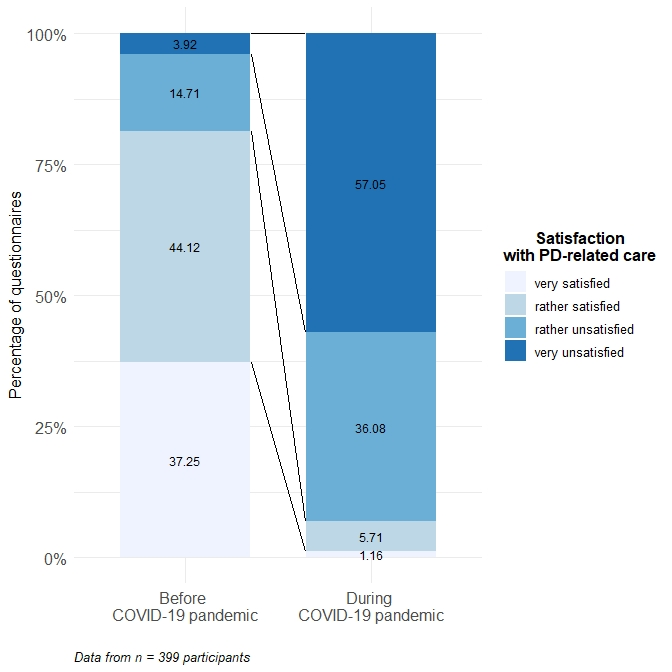
\includegraphics[width=.90\textwidth]{fig2.satisfaction.care.v1.0.jpeg}
\caption{Available questionnaires for this project}
\label{fig2:satisfaction}
\end{figure}

\begin{figure}
\centering
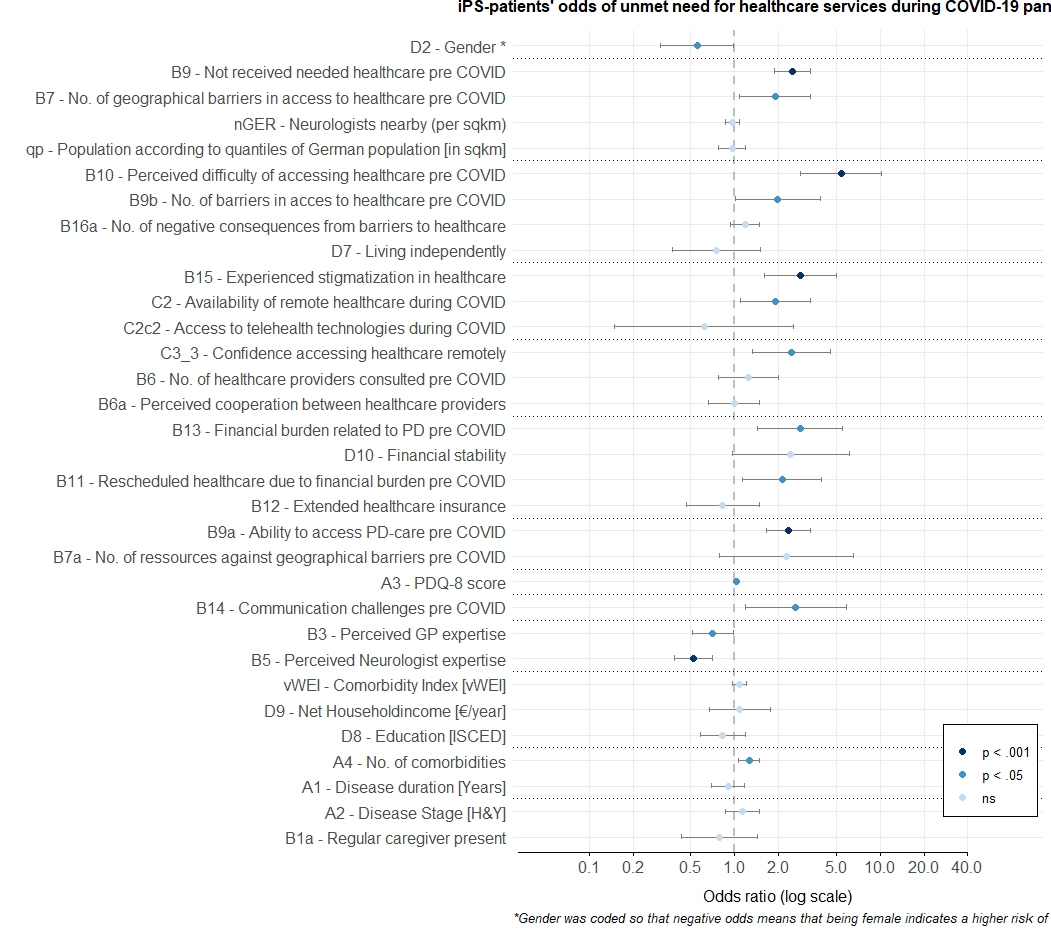
\includegraphics[width=.90\textwidth]{fig3.oddsratios.v1.0.jpeg}
\caption{Unadjusted Odds ratios according to the \textsc{GLM} for all 32 questions. Odds were determined so that higher values indicate affirmation to the question that healthcare was needed but this need remianed unmet during the COVID-19 pandemic. The dashed lines indicate the distinct domains according to ??, whereas significance is illustrated as color of the dot, with two distinct levels of significance. }%Quelle einfügen}
\label{fig3:resultsOR1}
\end{figure}




\newpage

	\section*{Discussion}
	Text for this section\ldots
	\section*{Conclusion}
	Text for this section\ldots
	\subsection*{Sub-heading for section}
	Text for this sub-heading\ldots
	\subsubsection*{Sub-sub heading for section}
	Text for this sub-sub-heading\ldots
	\paragraph*{Sub-sub-sub heading for section}
	Text for this sub-sub-sub-heading\ldots
	
	In this section we examine the growth rate of the mean of $Z_0$, $Z_1$ and $Z_2$. In
	addition, we examine a common modeling assumption and note the
	importance of considering the tails of the extinction time $T_x$ in
	studies of escape dynamics.
	We will first consider the expected resistant population at $vT_x$ for
	some $v>0$, (and temporarily assume $\alpha=0$)
	%
	\[
	E \bigl[Z_1(vT_x) \bigr]=
	\int_0^{v\wedge
		1}Z_0(uT_x)
	\exp (\lambda_1)\,du .
	\]
	%
	If we assume that sensitive cells follow a deterministic decay
	$Z_0(t)=xe^{\lambda_0 t}$ and approximate their extinction time as
	$T_x\approx-\frac{1}{\lambda_0}\log x$, then we can heuristically
	estimate the expected value as
	%
	\begin{equation}\label{eqexpmuts}
		\begin{aligned}[b]
			&      E\bigl[Z_1(vT_x)\bigr]\\
			&\quad      = \frac{\mu}{r}\log x
			\int_0^{v\wedge1}x^{1-u}x^{({\lambda_1}/{r})(v-u)}\,du .
		\end{aligned}
	\end{equation}
	%
	Thus we observe that this expected value is finite for all $v>0$ (also see \cite{koon,xjon,marg,schn,koha,issnic}).
	
	
	\section*{Appendix}
	Text for this section\ldots
	
	%%%%%%%%%%%%%%%%%%%%%%%%%%%%%%%%%%%%%%%%%%%%%%
	%%                                          %%
	%% Backmatter begins here                   %%
	%%                                          %%
	%%%%%%%%%%%%%%%%%%%%%%%%%%%%%%%%%%%%%%%%%%%%%%
	
	\begin{backmatter}
		
		\section*{Acknowledgements}%% if any
		Text for this section\ldots
		
		\section*{Funding}%% if any
		Text for this section\ldots
		
		\section*{Abbreviations}%% if any
		Text for this section\ldots
		
		\section*{Availability of data and materials}%% if any
		Text for this section\ldots
		
		\section*{Ethics approval and consent to participate}%% if any
		Text for this section\ldots
		
		\section*{Competing interests}
		The authors declare that they have no competing interests.
		
		\section*{Consent for publication}%% if any
		Text for this section\ldots
		
		\section*{Authors' contributions}
		Text for this section \ldots
		
		\section*{Authors' information}%% if any
		Text for this section\ldots
		
		%%%%%%%%%%%%%%%%%%%%%%%%%%%%%%%%%%%%%%%%%%%%%%%%%%%%%%%%%%%%%
		%%                  The Bibliography                       %%
		%%                                                         %%
		%%  Bmc_mathpys.bst  will be used to                       %%
		%%  create a .BBL file for submission.                     %%
		%%  After submission of the .TEX file,                     %%
		%%  you will be prompted to submit your .BBL file.         %%
		%%                                                         %%
		%%                                                         %%
		%%  Note that the displayed Bibliography will not          %%
		%%  necessarily be rendered by Latex exactly as specified  %%
		%%  in the online Instructions for Authors.                %%
		%%                                                         %%
		%%%%%%%%%%%%%%%%%%%%%%%%%%%%%%%%%%%%%%%%%%%%%%%%%%%%%%%%%%%%%
		\section*{References}
		% if your bibliography is in bibtex format, use those command
		
		\bibliographystyle{vancouver} % Style BST file (bmc-mathphys, vancouver, spbasic).
		\bibliography{bmc_article_covidPD}      % Bibliography file (usually '*.bib' )
		
		%%%%%%%%%%%%%%%%%%%%%%%%%%%%%%%%%%%
		%%                               %%
		%% Figures                       %%
		%%                               %%
		%% NB: this is for captions and  %%
		%% Titles. All graphics must be  %%
		%% submitted separately and NOT  %%
		%% included in the Tex document  %%
		%%                               %%
		%%%%%%%%%%%%%%%%%%%%%%%%%%%%%%%%%%%
		
		%%
		%% Do not use \listoffigures as most will included as separate files
		
		\section*{Figures}
		\begin{figure}[h!]
			\caption{Sample figure title}
		\end{figure}
		
		\begin{figure}[h!]
			\caption{Sample figure title}
		\end{figure}
		
		%%%%%%%%%%%%%%%%%%%%%%%%%%%%%%%%%%%
		%%                               %%
		%% Tables                        %%
		%%                               %%
		%%%%%%%%%%%%%%%%%%%%%%%%%%%%%%%%%%%
		
		%% Use of \listoftables is discouraged.
		%%
		\section*{Tables}
		\begin{table}[h!]
			\caption{Sample table title. This is where the description of the table should go}
			\begin{tabular}{cccc}
				\hline
				& B1  &B2   & B3\\ \hline
				A1 & 0.1 & 0.2 & 0.3\\
				A2 & ... & ..  & .\\
				A3 & ..  & .   & .\\ \hline
			\end{tabular}
		\end{table}
		
		%%%%%%%%%%%%%%%%%%%%%%%%%%%%%%%%%%%
		%%                               %%
		%% Additional Files              %%
		%%                               %%
		%%%%%%%%%%%%%%%%%%%%%%%%%%%%%%%%%%%
		
		\section*{Additional Files}
		\subsection*{Additional file 1 --- Sample additional file title}
		Additional file descriptions text (including details of how to
		view the file, if it is in a non-standard format or the file extension).  This might
		refer to a multi-page table or a figure.
		
		\subsection*{Additional file 2 --- Sample additional file title}
		Additional file descriptions text.
	\end{backmatter}
\end{document}
